\documentclass[tikz, border=2mm]{standalone} 
\usepackage{amsmath}
\usepackage{graphicx}
\usepackage{bm} % For bold math symbols
\usetikzlibrary{arrows.meta, decorations.pathreplacing, calc} 

% Define colors
\definecolor{myblue}{RGB}{15, 133, 165}
\definecolor{myred}{RGB}{187, 37, 66}
\definecolor{mydark}{RGB}{20, 25, 45}
\definecolor{samyellow}{RGB}{250, 240, 100}
\definecolor{sampurple}{RGB}{210, 80, 220}

% Soft pastel colors for the background boxes
\definecolor{boxblue}{RGB}{225, 238, 245}
\definecolor{boxyellow}{RGB}{252, 235, 170}

% Macros for styled dots
\def\ydot#1#2{
    \fill[black, opacity=0.15] (#1+0.15, #2+0.15) circle (0.8);
    \fill[samyellow, opacity=1] (#1, #2) circle (0.8);
}
\def\pdot#1#2{
    \fill[black, opacity=0.15] (#1+0.15, #2+0.15) circle (0.7);
    \fill[sampurple, opacity=1] (#1, #2) circle (0.7);
}

% Reusable drawing macros
\newcommand{\drawtriangles}{
    \fill[myblue, opacity=0.85] (2, 11) -- (16, 2) -- (20, 19) -- cycle;
    \fill[myred, opacity=0.85] (10, 12) -- (26, 1) -- (31, 16) -- cycle;
}

\newcommand{\drawghost}{
    \begin{scope}[shift={(0, -2)}]
        \fill[myblue, opacity=0.4] (2, 11) -- (16, 2) -- (20, 19) -- cycle;
    \end{scope}
}

\newcommand{\drawcircle}{
    \draw[mydark, dashed, line width=3pt, dash pattern=on 8pt off 8pt] 
        (15.5, 7.5) circle (6);
}

\newcommand{\drawhighlights}{
    \draw[sampurple, line width=5.5pt, opacity=0.45, line join=round] (2, 11) -- (16, 2) -- (20, 19) -- cycle;
    \draw[sampurple, line width=5.5pt, opacity=0.45, line join=round] (10, 12) -- (26, 1) -- (31, 16) -- cycle;
}

% A mathematically perfect rectangle aligned to the edge and the normal.
\newcommand{\drawpurplerect}{
    % Length is parallel to the edge, width is parallel to the normal n
    \fill[sampurple, opacity=0.7] (13.854, 9.342) -- (17.146, 7.078) -- (15.982, 5.386) -- (12.690, 7.650) -- cycle;
    \pdot{15.5}{8.21} % Perfectly centered in the rectangle
}

% --- TIGHT BOUNDING BOX MACRO ---
\newcommand{\tightboundingbox}{
    \useasboundingbox (0.5, -1.5) rectangle (33.5, 19.2);
}

\begin{document}

% ==========================================
% PAGE 1
% ==========================================

\begin{tikzpicture}[y=-1cm, scale=0.4]
    \tightboundingbox
    \drawtriangles
\end{tikzpicture}

% ==========================================
% PAGE 2
% ==========================================
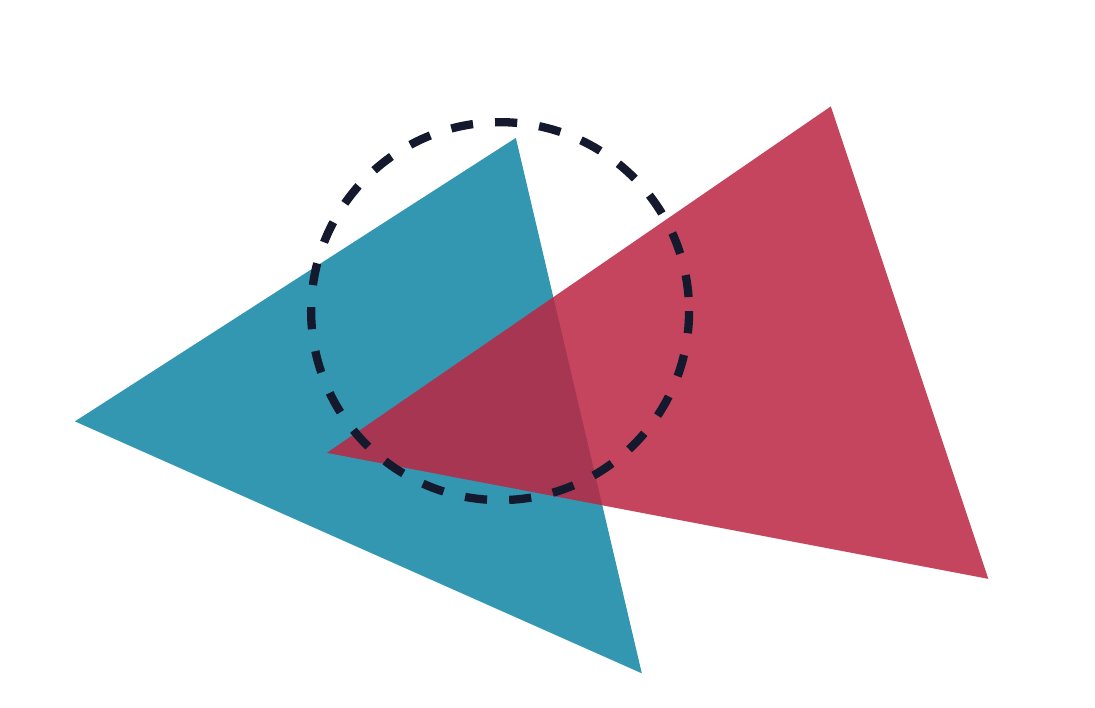
\begin{tikzpicture}[y=-1cm, scale=0.4]
    \tightboundingbox
    \drawtriangles
    \drawcircle
\end{tikzpicture}

% ==========================================
% PAGE 3
% ==========================================
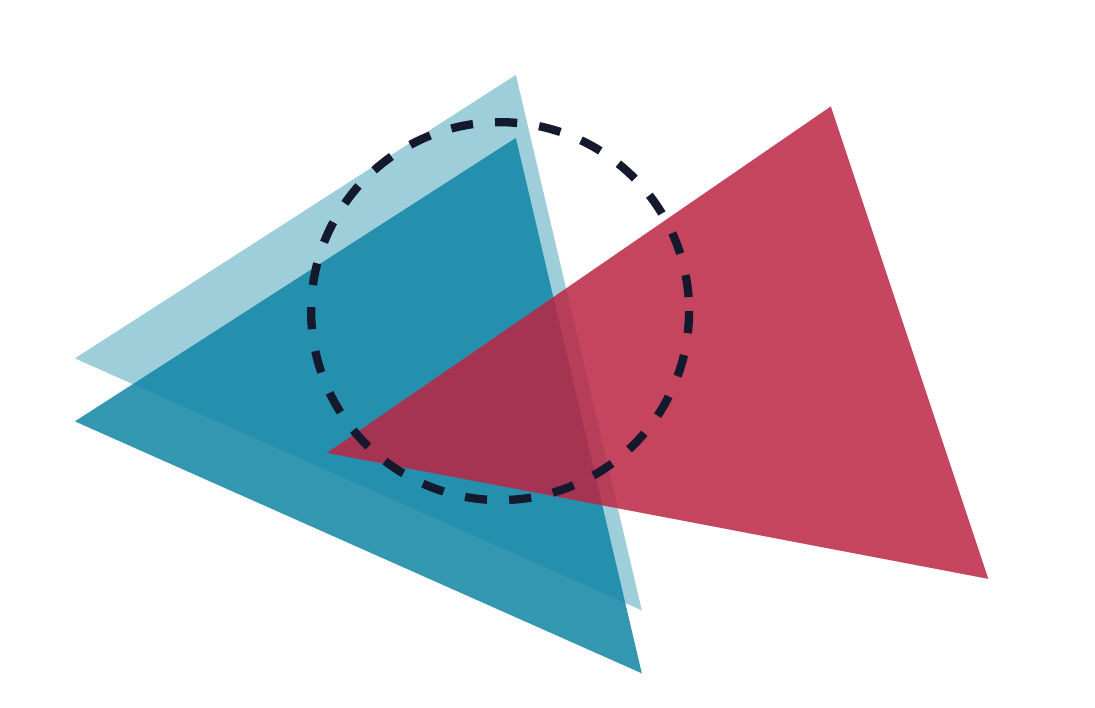
\begin{tikzpicture}[y=-1cm, scale=0.4]
    \tightboundingbox
    \drawghost
    \drawtriangles
    \drawcircle
\end{tikzpicture}

% ==========================================
% PAGE 3b
% ==========================================
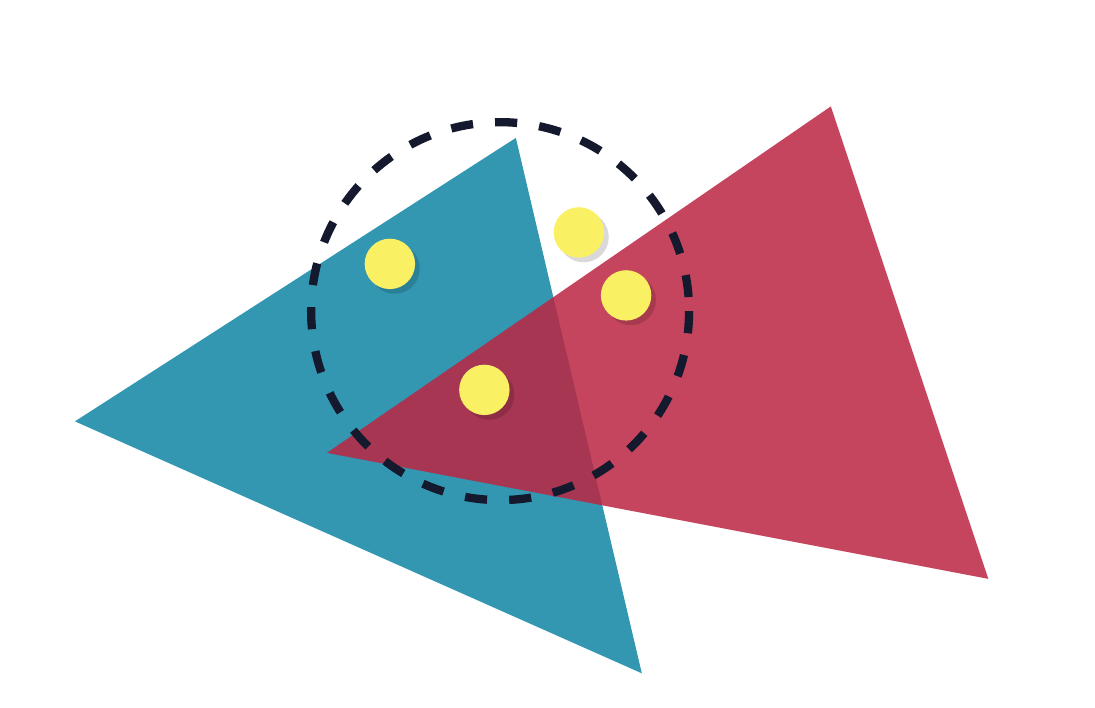
\begin{tikzpicture}[y=-1cm, scale=0.4]
    \tightboundingbox
    \drawtriangles
    \drawcircle
    \ydot{12}{6} \ydot{18}{5} \ydot{15}{10} \ydot{19.5}{7}
\end{tikzpicture}

% ==========================================
% PAGE 4
% ==========================================
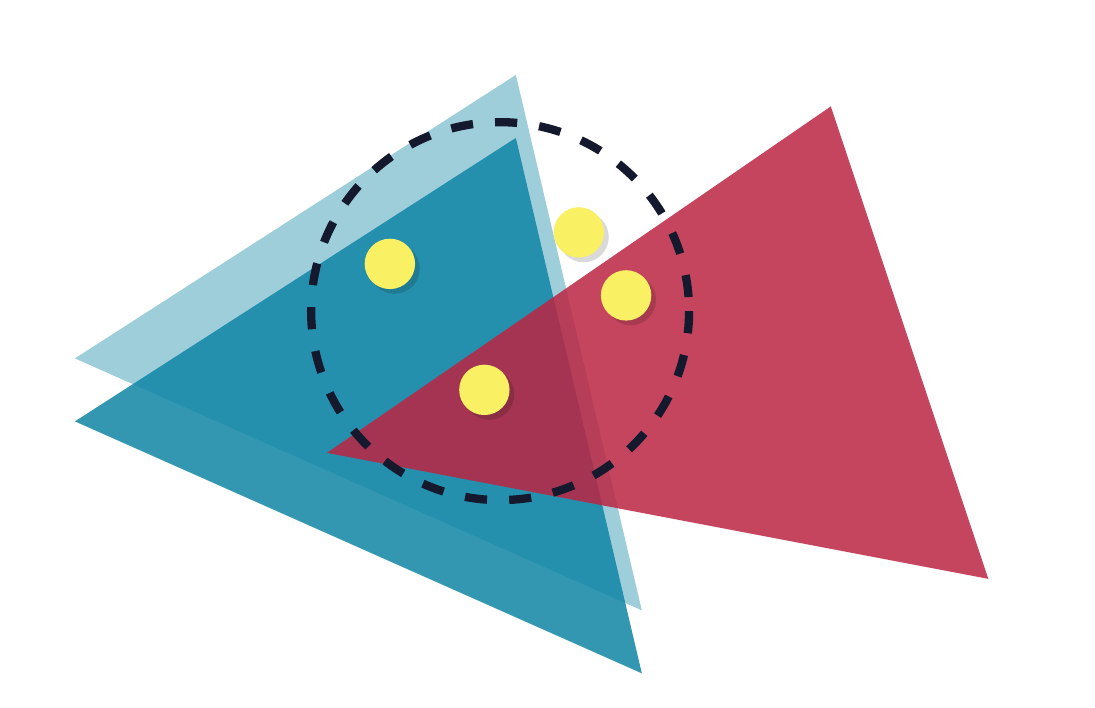
\begin{tikzpicture}[y=-1cm, scale=0.4]
    \tightboundingbox
    \drawghost
    \drawtriangles
    \drawcircle
    \ydot{12}{6} \ydot{18}{5} \ydot{15}{10} \ydot{19.5}{7}
\end{tikzpicture}

% ==========================================
% PAGE 5
% ==========================================
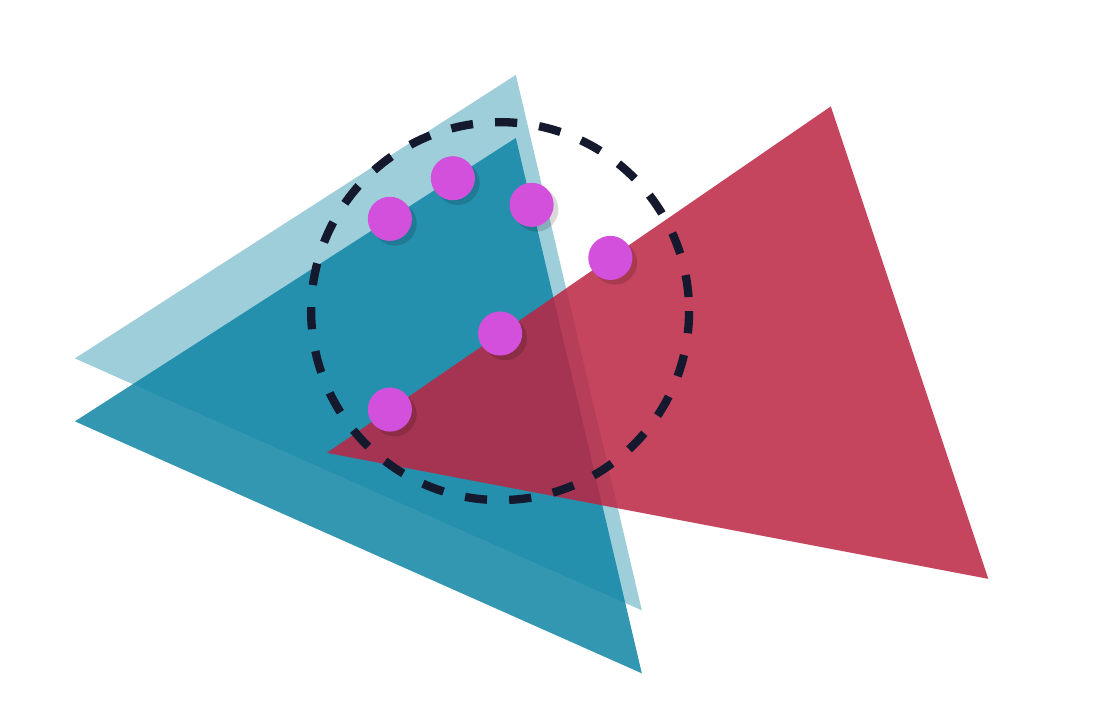
\begin{tikzpicture}[y=-1cm, scale=0.4]
    \tightboundingbox
    \drawghost
    \drawtriangles
    \drawcircle
    \pdot{12}{10.625} \pdot{15.5}{8.21} \pdot{19}{5.81}
    \pdot{12}{4.57} \pdot{14}{3.28} \pdot{16.5}{4.125}
\end{tikzpicture}

% ==========================================
% PAGE 6
% ==========================================
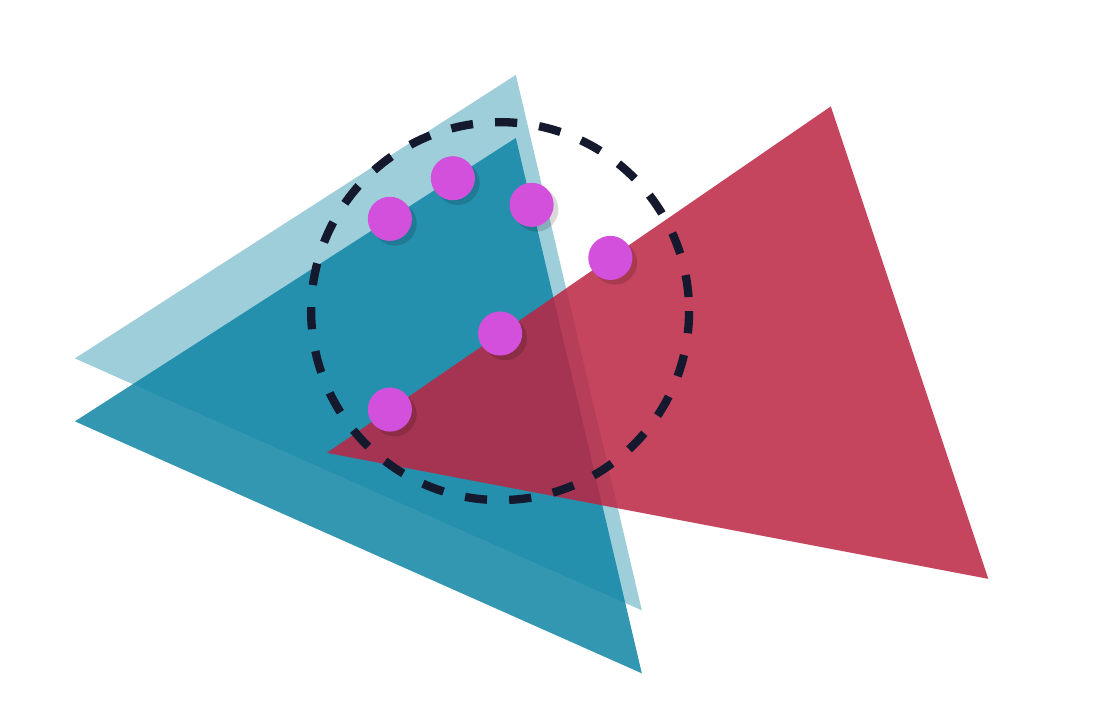
\begin{tikzpicture}[y=-1cm, scale=0.4]
    \tightboundingbox
    \drawghost
    \drawtriangles
    \drawcircle
    \pdot{12}{10.625} \pdot{15.5}{8.21} \pdot{19}{5.81}
    \pdot{12}{4.57} \pdot{14}{3.28} \pdot{16.5}{4.125}
\end{tikzpicture}


% ==========================================
% PAGE 7: Full Equation
% ==========================================
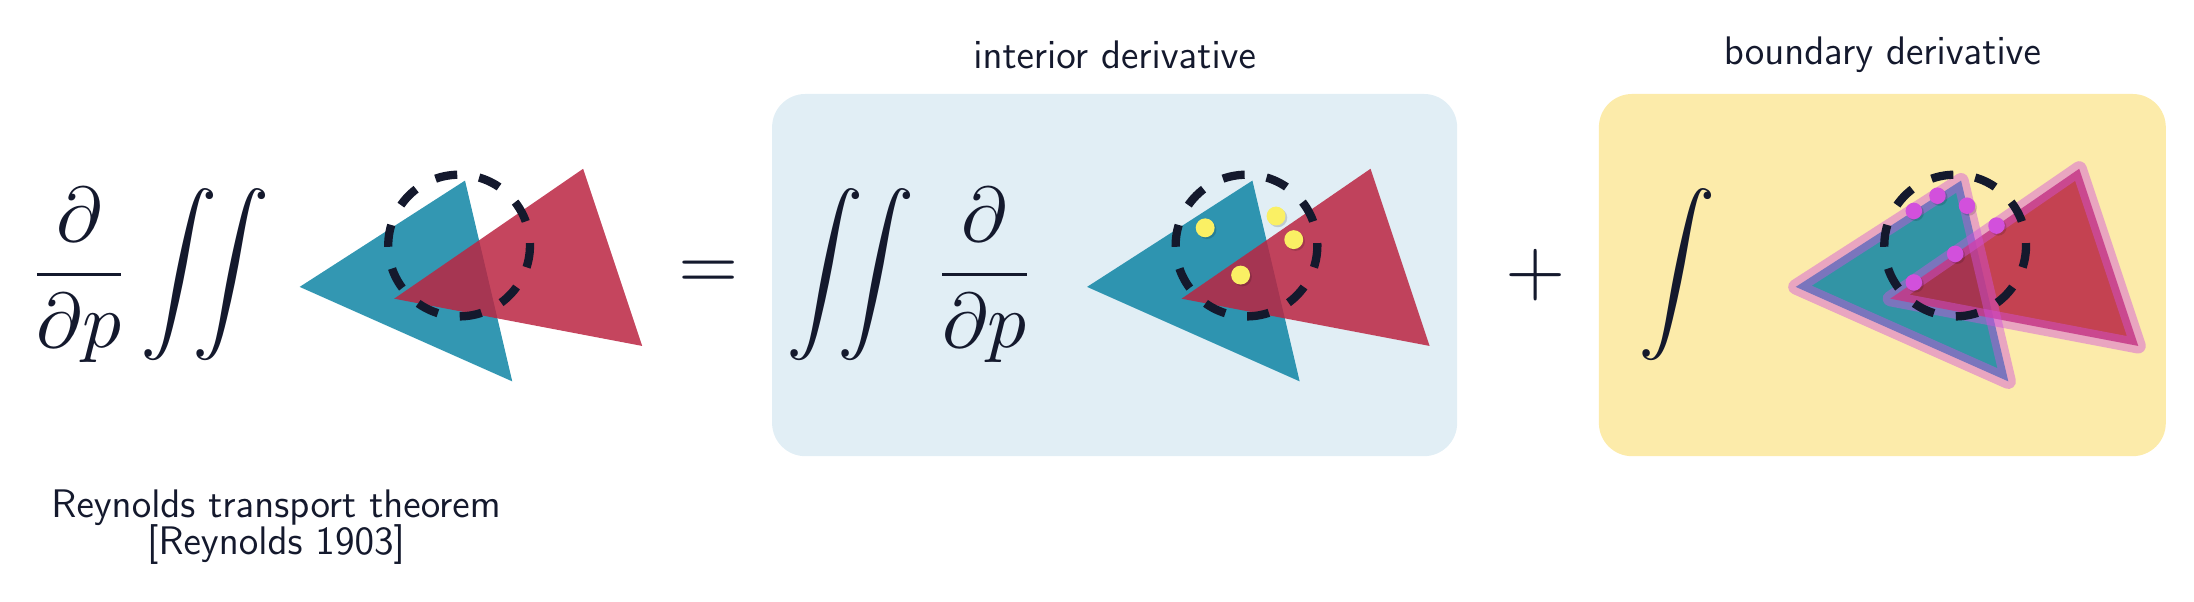
\begin{tikzpicture}[y=-1cm, font=\sffamily]
\tikzset{mathnode/.style={anchor=center, inner sep=0, mydark}}

\node[mathnode] at (0, 0) {\scalebox{2.8}{$\displaystyle \frac{\partial}{\partial p}$}};
\node[mathnode] at (1.6, 0) {\scalebox{2.8}{$\displaystyle \iint$}};

\begin{scope}[shift={(2.5, -1.5)}, scale=0.15]
    \drawtriangles
    \drawcircle
\end{scope}

\node[mathnode] at (8, 0) {\scalebox{2.8}{$=$}};

\fill[boxblue, rounded corners=12pt] (8.8, -2.3) rectangle (17.5, 2.3);
\node[mydark] at (13.15, -2.8) {\Large interior derivative};

\node[mathnode] at (9.8, 0) {\scalebox{2.8}{$\displaystyle \iint$}};
\node[mathnode] at (11.5, 0) {\scalebox{2.8}{$\displaystyle \frac{\partial}{\partial p}$}};

\begin{scope}[shift={(12.5, -1.5)}, scale=0.15]
    \drawtriangles
    \drawcircle
    \ydot{12}{6} \ydot{18}{5} \ydot{15}{10} \ydot{19.5}{7}
\end{scope}

\node[mathnode] at (18.5, 0) {\scalebox{2.8}{$+$}};

\fill[boxyellow, rounded corners=12pt] (19.3, -2.3) rectangle (26.5, 2.3);
\node[mydark] at (22.9, -2.8) {\Large boundary derivative};

\node[mathnode] at (20.3, 0) {\scalebox{2.8}{$\displaystyle \int$}};

\begin{scope}[shift={(21.5, -1.5)}, scale=0.15]
    \drawtriangles
    \drawhighlights
    \drawcircle
    \pdot{12}{10.625} \pdot{15.5}{8.21} \pdot{19}{5.81}
    \pdot{12}{4.57} \pdot{14}{3.28} \pdot{16.5}{4.125}
\end{scope}

\node[align=center, mydark] at (2.5, 3.2) {\Large Reynolds transport theorem\\[-0.1em] \Large[Reynolds 1903]};
\end{tikzpicture}


% ==========================================
% PAGE 8: Movement on RED Triangle + Zoom
% ==========================================
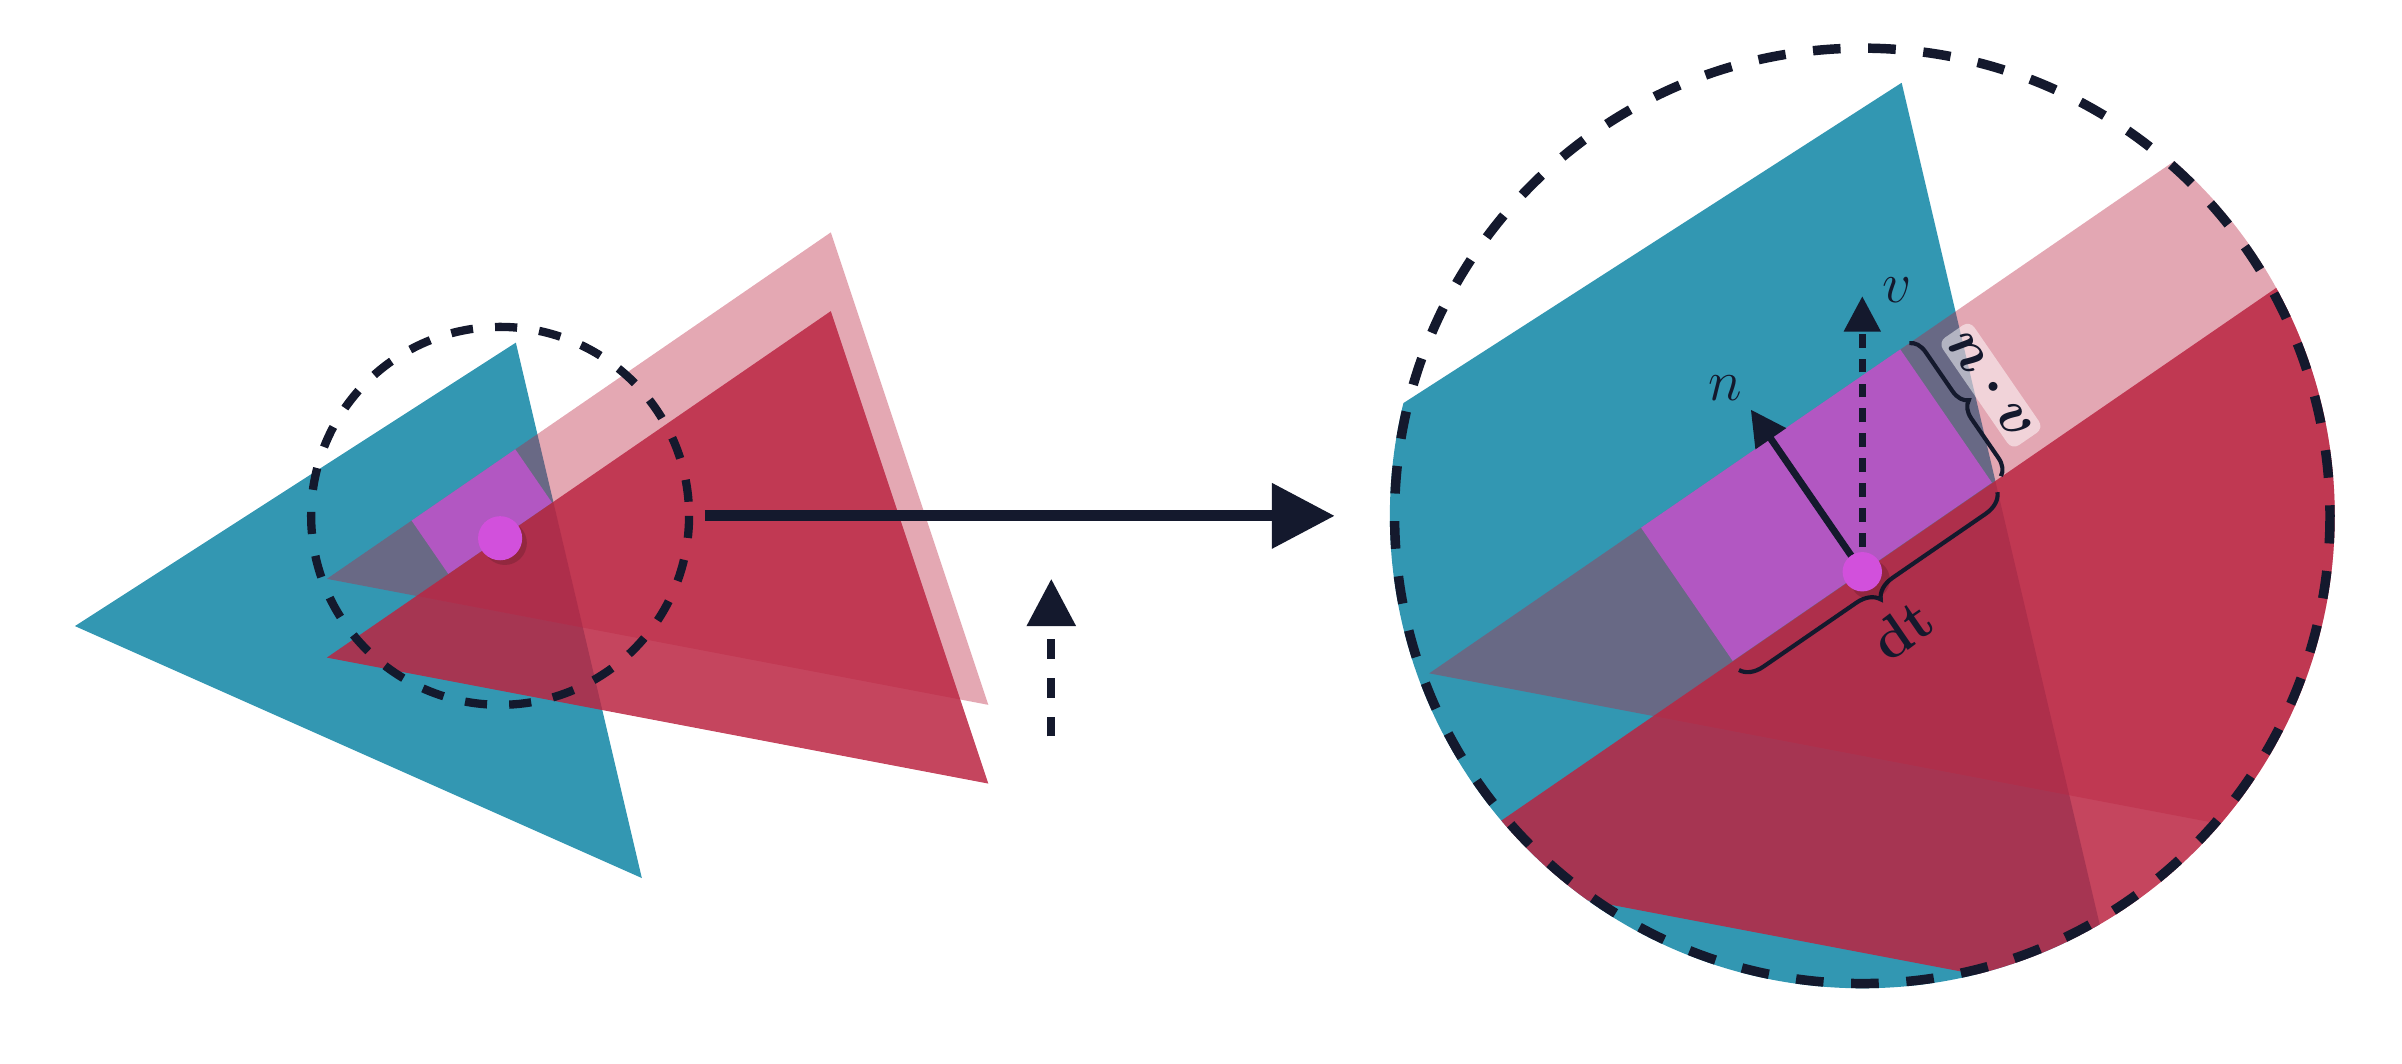
\begin{tikzpicture}[y=-1cm, scale=0.4]
    % Wide bounding box to hold both the original image and the zoomed version
    \useasboundingbox (0.5, -8) rectangle (75, 24);
    
    % ----------------------------------------------------
    % LEFT HALF: Base Overview Graphic
    % ----------------------------------------------------
    \fill[myblue, opacity=0.85] (2, 11) -- (16, 2) -- (20, 19) -- cycle;
    \begin{scope}[shift={(0, -2.5)}]
        \fill[myred, opacity=0.4] (10, 12) -- (26, 1) -- (31, 16) -- cycle;
    \end{scope}
    \fill[myred, opacity=0.85] (10, 12) -- (26, 1) -- (31, 16) -- cycle;
    
    \drawcircle
    \drawpurplerect

    % Movement upward arrow
    \draw[-{Triangle[length=6mm, width=6mm]}, dashed, line width=3pt, mydark, dash pattern=on 7pt off 7pt] 
        (33, 14.5) -- (33, 9.5);

    % Connection Arrow pointing to the Zoomed right half
    \draw[-{Triangle[length=8mm, width=8mm]}, line width=4pt, mydark] (22, 7.5) -- (42, 7.5);


    % ----------------------------------------------------
    % RIGHT HALF: High-Resolution Zoomed Pixel Support
    % ----------------------------------------------------
    % Scaled by 2.5 and shifted perfectly inline with the left circle
    \begin{scope}[shift={(20, -11.25)}, scale=2.5, font=\sffamily]
        
        % 1. Clip everything outside the local pixel support circle
        \clip (15.5, 7.5) circle (6);
        
        % Solid white background inside the circle for a clean cutout
        \fill[white] (9, 1) rectangle (22, 14);

        % 2. Solid Blue Triangle
        \fill[myblue, opacity=0.85] (2, 11) -- (16, 2) -- (20, 19) -- cycle;
        
        % 3. Ghost Red Triangle (Shifted)
        \begin{scope}[shift={(0, -2.5)}]
            \fill[myred, opacity=0.4] (10, 12) -- (26, 1) -- (31, 16) -- cycle;
        \end{scope}
        
        % 4. Solid Red Triangle
        \fill[myred, opacity=0.85] (10, 12) -- (26, 1) -- (31, 16) -- cycle;

        % 5. Swept Purple Rectangle 
        \fill[sampurple, opacity=0.7] (13.854, 9.342) -- (17.146, 7.078) -- (15.982, 5.386) -- (12.690, 7.650) -- cycle;

        % 6. Annotations: Curly Braces
        % Length Brace (Bottom Edge - Mirror forces it outward)
        \draw[mydark, decorate, decoration={brace, amplitude=8pt, raise=4pt, mirror}, line width=1.5pt] 
            (13.854, 9.342) -- (17.146, 7.078) node[midway, sloped, below=14pt] {\huge $\mathbf{dt}$};
            
        % Width Brace (Right Edge)
        \draw[mydark, decorate, decoration={brace, amplitude=6pt, raise=4pt}, line width=1.5pt] 
            (15.982, 5.386) -- (17.146, 7.078) 
            node[midway, sloped, above=12pt, fill=white, fill opacity=0.5, text opacity=1, inner sep=2pt, rounded corners=3pt] {\huge $\bm{n \cdot v}$};

        % 7. Sample Point Coordinate (Center of the swept rectangle base)
        \coordinate (P) at (15.5, 8.21);

        % 8. Vectors
        % Normal vector (n): Mathematically perpendicular to the edge
        \draw[-{Triangle[length=4.5mm, width=4.5mm]}, line width=2.5pt, mydark] 
            (P) -- ++(-124.5085:2.5) node[above left, inner sep=2pt] {\huge $n$};
            
        % Velocity vector (v): Straight up 
        \draw[-{Triangle[length=4.5mm, width=4.5mm]}, dashed, dash pattern=on 5pt off 4pt, line width=2.5pt, mydark] 
            (P) -- ++(0, -3.5) node[right, inner sep=6pt, yshift=2pt] {\huge $v$};

        % 9. Sample Point Dot 
        \fill[black, opacity=0.15] ($(P)+(0.1, 0.1)$) circle (0.25);
        \fill[sampurple] (P) circle (0.25);

        % 10. Pixel Support Circle Boundary
        \draw[mydark, dashed, line width=4pt, dash pattern=on 10pt off 10pt] 
            (15.5, 7.5) circle (5.95);
            
    \end{scope}

\end{tikzpicture}

\end{document}